\documentclass[11pt,letterpaper]{article}
\usepackage[margin=.7in]{geometry}
\usepackage{graphicx,xcolor}
\setlength{\parindent}{0pt}
\begin{document}
{\sffamily\Large\bfseries Crossed-box circles: exact user example}\par\medskip
Same diagram, options and display scale. Only the package code changes.
\par\vspace{24pt}
\begin{minipage}[t]{.48\linewidth}\centering
{\sffamily\bfseries Before}\par\bigskip
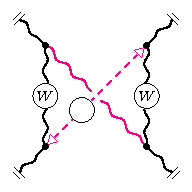
\includegraphics[width=.95\linewidth]{../../../docs/planning/reproductions/d02-cross-box-circles-before.pdf}\par\medskip
Three circles: two W rings plus an unwanted empty Proca ring.
\par\medskip
Requested \texttt{circ scale=0.6} is ignored.\par
W-ring radius: 5.978 PDF pt.
\end{minipage}\hfill
\begin{minipage}[t]{.48\linewidth}\centering
{\sffamily\bfseries After}\par\bigskip
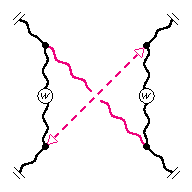
\includegraphics[width=.95\linewidth]{../../../docs/planning/reproductions/d02-cross-box-circles-after.pdf}\par\medskip
Two explicitly requested W rings. The bare pink Proca line has no circle.
\par\medskip
\texttt{circ scale=0.6} scales both ring and W text.\par
W-ring radius: 3.587 PDF pt.
\end{minipage}
\par\vspace{30pt}
{\sffamily\bfseries Verified behavior}\par\medskip
Both internal crossed-box layouts preserve line-local circle sizes and colors.
Explicit Proca circles still work, including one circle on a split line.
The crossing gap and endpoint markers are unchanged.
\par\medskip
Source: the user's unchanged \texttt{CrossBoxCorr} options, saved in the D02
reproducer. The before output uses package checkpoint \texttt{e64cc2f};
the after output uses the corrected package.
\end{document}
